\documentclass[10pt,dvipdfmx]{jsarticle}
\usepackage{ascmac}
\usepackage[margin=15truemm]{geometry}
\usepackage{amsmath}
\usepackage[dvipdfmx]{graphicx}
\usepackage{subcaption}
\setlength{\columnseprule}{0.3mm}


\begin{document}

\title{信号処理特論 第12回課題}
\author{視覚認知システム研究室\\学籍番号:2433730032 岡村 翼}
\date{\today}
\maketitle

{\textgt{課題} }
課題1のインパルス入力を左図上、ステップ入力を図\ref{fig:impulse}に示す。\\
課題2の原信号、単純移動平均法、2次多項式適合法の順にグラフ化したものを図\ref{fig:moving}に示す。\\
  \begin{figure}[h]
    \centering
      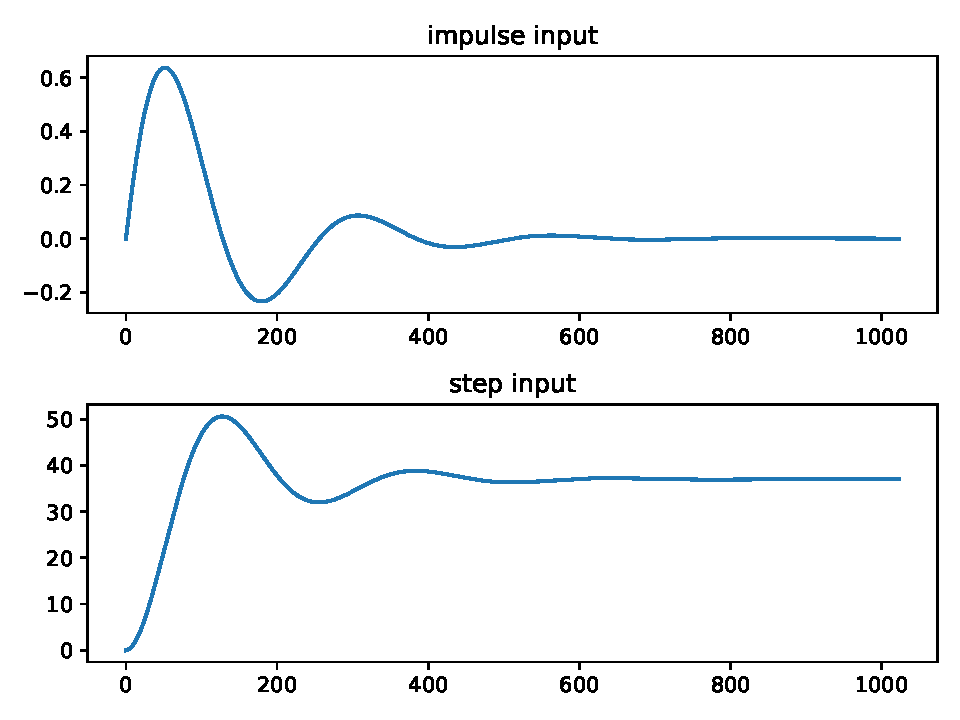
\includegraphics[width=0.8\textwidth]{impulse.pdf}
	\caption{impulse}
      \label{fig:impulse}
 \end{figure}
  \begin{figure}[h]
  \centering
      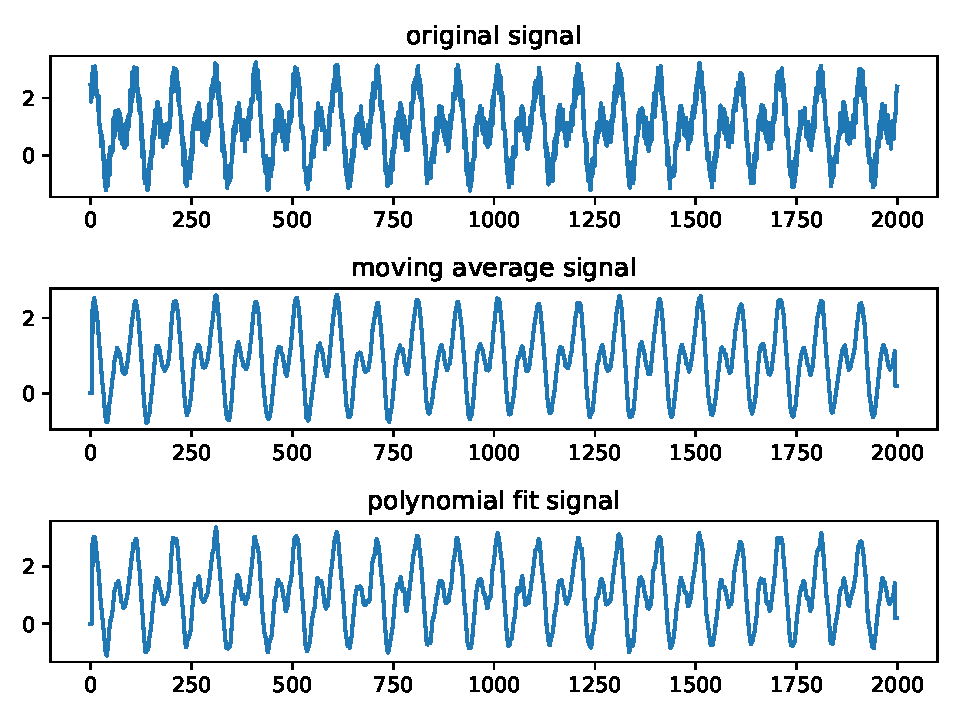
\includegraphics[width=0.8\textwidth]{moving_average.pdf}
	\caption{moving average}
      \label{fig:moving}
 \end{figure}
\end{document}